\chapter{Data Analysis and Pre-processing}
\label{Ch:Data}
\section{Data descripcion}

The dataset consists of two FITS files corresponding to the simulated observations of the DESI instrument and the "truth" data from cosmological simulations. Each data file has a key column called TARGETID, this variables is the same across all simulations and identifies a particular object in the sky, thus it is needed to relate both datasets. 
\subsection{Simulated expected results - truth file}
This file contains the data from the cosmological simulation of the target objects. Thus, this file contains the expected redshift that the instrument \textit{should} measure. The complete list of columns in the file is shown in table \ref{tab:true_car}\footnote{Additional information on \url{https://desidatamodel.readthedocs.io/en/stable/}}. Since we aim to correct the measurements of redshifts given by the instrument, the variable TRUEZ will be our target variable or "\textit{output}" to the machine learning models. The rest of the information will be used mostly for understanding the dataset but no as part of the ML model since this information would not be available to the instrument in reality. This dataset contains the redshift of 24.851.543 objects. 
\begin{table}[!htbp]
	\centering
	\begin{tabular}{c}
		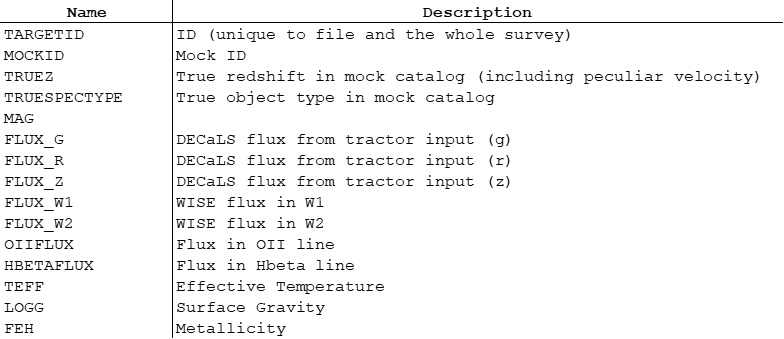
\includegraphics[width=0.9\linewidth]{TeX_files/Imagenes/Imagen2}
	\end{tabular} 
	\caption{Columns in the cosmological simulation data file}
	\label{tab:true_car}
\end{table}
\subsection{Simulated Observations - target file}
This file contains the redshift values of the targets as measured by the instrument in simulation. Apart from this, it also contains the columns shown in table \ref{tab:tar_car}. The different characteristics listed in Table \ref{tab:tar_car} are the ones that we will use as input in our machine learning models, since is the data available from the instrument. This dataset contains the redshift of 2.131.896 objects. 
\begin{table}[!htbp]
	\centering
	\begin{tabular}{c}
		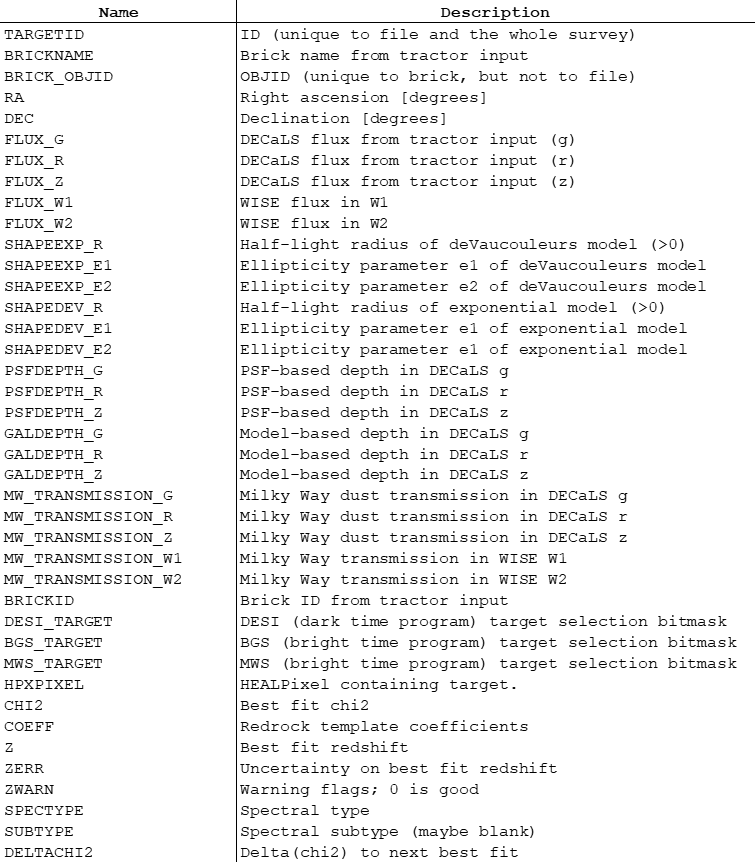
\includegraphics[width=0.9\linewidth]{TeX_files/Imagenes/Imagen1}    
	\end{tabular} 
	\caption{Columns in the Simulated Observations data file }
	\label{tab:tar_car}
\end{table}
Since the files don´t have the same amount of points, they were cut to the one with the least (the target file) by linking the rows by its TARGETID. 
\section{Overview of the dataset}
\subsection{Redshift relations}
To understand the dataset, the first thing we need to do is see how the Z and TRUEZ variables behave. In Figure \ref{fig:z-truez} we see three distinct regions: a 45-degree line that corresponds to the redshifts measurements of DESI that are very close to the expected 'real' value, a square region where the data seems to scatter randomly except for some line groupings, and a third region of horizontal line near True Z = 0. The task is, therefore, to dissolve the square region and have all the points along the diagonal line.   
\begin{figure}[h!]
	\centering
	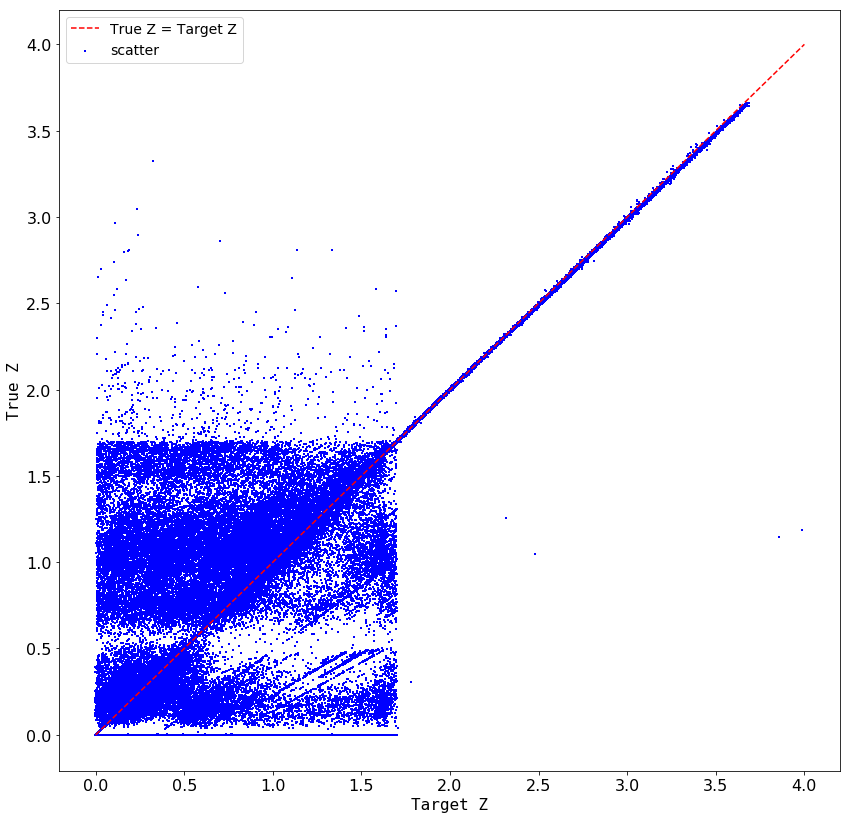
\includegraphics[width=1.0\linewidth]{TeX_files/Imagenes/z-truez}
	\caption{Relation between the 'observed' readshift - target Z, and the 'generated' redshift - True Z.}
	\label{fig:z-truez}
\end{figure}

Now, cutting along the MAG (magnitude) variable, it is possible to see the distribution of magnitudes of the gathered data an see if there is any relation with the square region. Figure \ref{fig:mag-dist} shows this distribution and Figure \ref{fig:mag-prop-dist} shows the fraction redshifts of each bin that is within a 1\% error of the true value. We can see that the majority of the redshift is near its true value, however, some valleys indicate that some regions (for example between 15 and 17 in magnitude) are not that good. For simplicity, from now on we will refer to the \textbf{simulated expected redshift} as TRUEZ (the output to the ML models) and the \textbf{simulated observations of the targets} as Z (the input to the models) or TARZ.
\begin{figure}
	\centering
	\begin{subfigure}[b]{1.0\textwidth}
		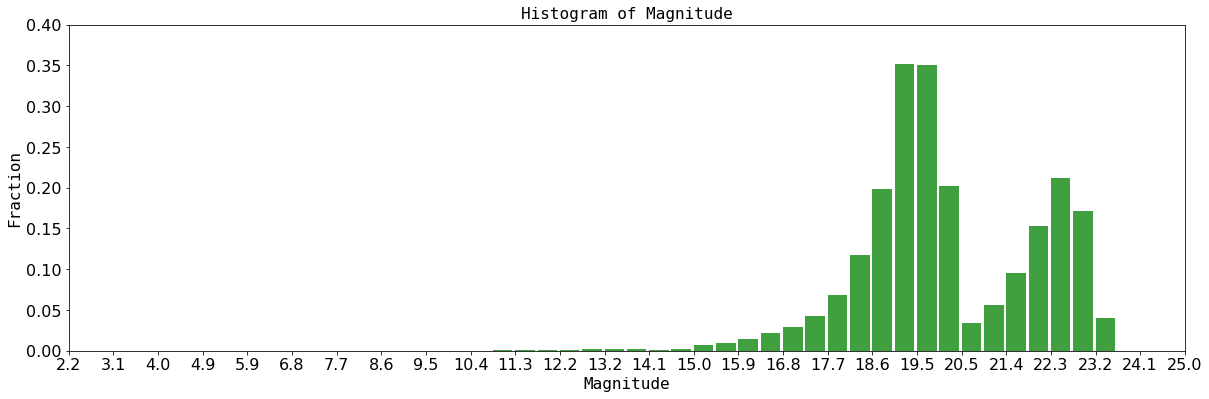
\includegraphics[width=1\linewidth]{TeX_files/Imagenes/mag-dist}
		\caption{}
		\label{fig:mag-dist} 
	\end{subfigure}    
	\begin{subfigure}[b]{1.0\textwidth}
		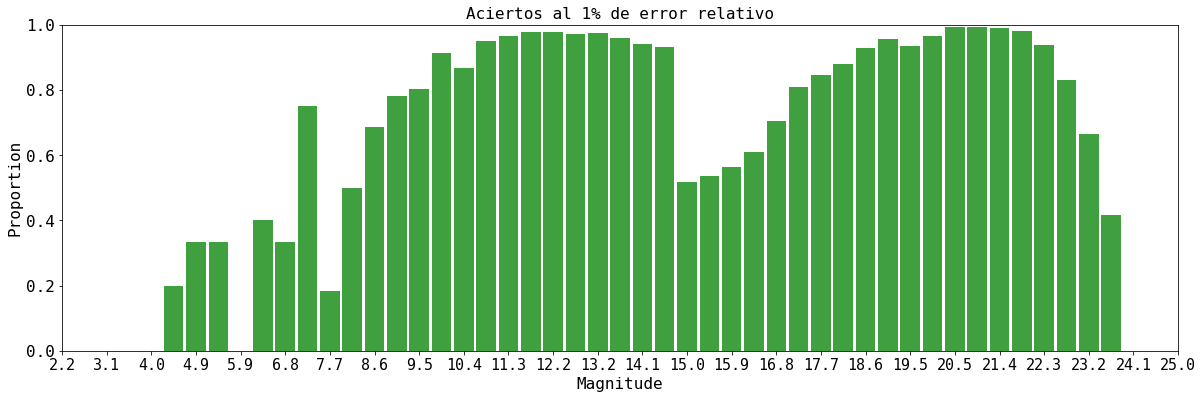
\includegraphics[width=1\linewidth]{TeX_files/Imagenes/mag-prop-dist}
		\caption{}
		\label{fig:mag-prop-dist}
	\end{subfigure}
	\caption{(a) Distribution of magnitudes in the dataset. (b) Proportion of the number of measured redshifts that are within the 1\% error of their corresponding TRUEZ }
	\label{fig:mag-dist-both}
\end{figure}
\subsection{Spectral types}
From figure \ref{fig:mag-dist-both} it is possible to infer that the different magnitudes of the targets can be related to the different regions on figure \ref{fig:z-truez}, and this difference in magnitude is also related to the SPECTYPE of each target. The spectral type of the data in the tar-file is distributed as shown in Table \ref{tab:espectype-N}. Near 85\% of the dataset is composed of Galaxy-type objects, for this reason, this is the most interesting class.
\begin{table}[!h]
	\centering
	\begin{tabular}{c|c|c}
		
		SPECTYPE & N samples & \% of dataset \\ 
		\hline 
		Galaxy & 1796213 & 84.25 \\ 
		
		QSO & 194319 & 9.11 \\ 
		
		Star & 141364 & 6.63 \\ 
		
		Total & 2131896 & 100 \\ 
		
	\end{tabular} 
	\caption{Spectral type distribution of the tar file. }
	\label{tab:espectype-N}
\end{table}
\begin{figure}
	\centering
	\begin{subfigure}[b]{0.5\textwidth}
		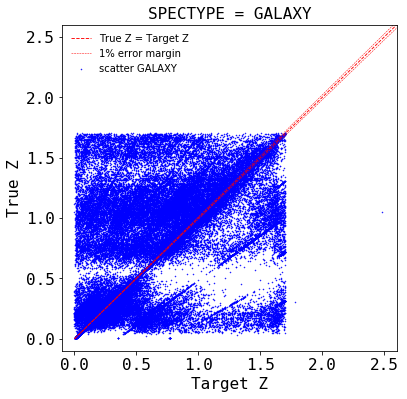
\includegraphics[width=1\linewidth]{TeX_files/Imagenes/GALAXY-z-truez}
		\caption{}
		\label{fig:GALAXY-z-truez} 
	\end{subfigure}    
	\begin{subfigure}[b]{0.5\textwidth}
		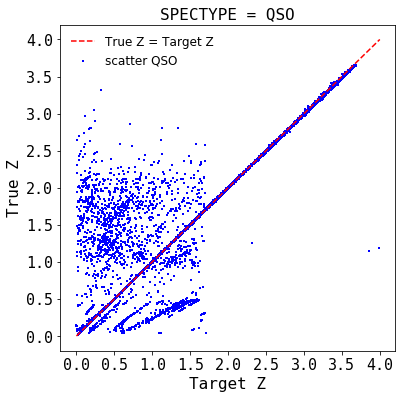
\includegraphics[width=1\linewidth]{TeX_files/Imagenes/QSO-z-truez}
		\caption{}
		\label{fig:QSO-z-truez}
	\end{subfigure}
	\begin{subfigure}[b]{0.5\textwidth}
		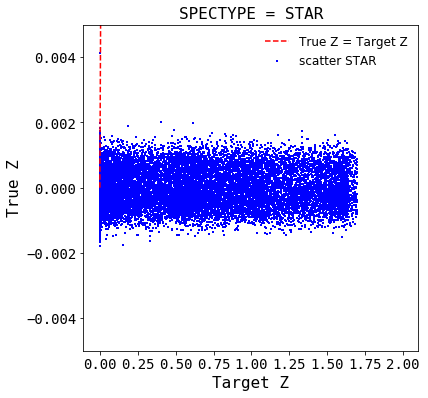
\includegraphics[width=1\linewidth]{TeX_files/Imagenes/STAR-z-truez}
		\caption{}
		\label{fig:STAR-z-truez}
	\end{subfigure}
	\caption{ Redshift relation for (a) Galaxy-type objects, (b) QSO-type objects, and (c) Star-type objects }
	\label{fig:SPECTYPE-z-truez}
\end{figure}

The redshift relations similar to Figure \ref{fig:z-truez} discriminated by SPECTYPE are shown in Figure \ref{fig:SPECTYPE-z-truez}, where the three regions in Figure \ref{fig:z-truez} seems to be related to each spectral type. The GALAXY objects are distributed along a square and there are lines formed at angles different than 45, which means that there is a relation between the two variable but 'out of calibration'. It is worth mentioning that Figure \ref{fig:GALAXY-z-truez}  can be deceiving because 96.34\% of the Galaxy-type data is within the 1\% margin line in the figure, which means that the square is formed only by the 3.66 \% of the galaxy data, corresponding to approximately  65.742 measurements, still a lot. 

The QSO-type objects in Figure \ref{fig:QSO-z-truez} correspond to the 45-degree line in Figure \ref{fig:z-truez} since the majority of points are along this line, although the same line pattern and dispersion of the galaxy-type objects are present, in the least quantity. However, the Star-type in Figure \ref{fig:STAR-z-truez} is randomly scattered over the TARZ range and correspond to the horizontal line in Figure \ref{fig:z-truez}. Once again, the most interesting SPECTYPE is GALAXY, because it has the majority of error in TARZ, and also presents different patterns, QSOs are already fine and are not a priority while STAR is completely random a represent a small fraction of the whole dataset. From now on we will focus on Galaxy-type objects only.  

\subsection{Galaxy-type objects}
Galaxy-type objects are classified as Bright Galaxy Survey (BGS), Emission Line Galaxies (ELG) and Luminous Red Galaxies (LRG) distributing according to Table \ref{tab:Galaxy-sub-types}. In this case, the sub-types are more evenly distributed. The redshift relations of each sub-type is shown in Figure \ref{fig:GALAXY-SUB-z-truez}. BGS and ELG follow a similar pattern, however, ELG is more disperse while BGS is clustered along the TARZ = TRUEZ line, whereas LRG sub-type is already perfect. 
\begin{table}[!h]
	\centering
	\begin{tabular}{c|c|c}
		Galaxy subtype & N samples  & \% of dataset  \\ 
		\hline 
		BGS & 889336 & 49.51 \\      
		ELG & 601847 & 33.51 \\  
		LRG & 305030 & 16.98 \\ 
		Total & 1796213 & 100 \\  
	\end{tabular} 
	\caption{Distribution of Galaxy sub-types}
	\label{tab:Galaxy-sub-types}
\end{table}

Note that the line structures are more visible in Figure \ref{fig:BGS-z-truez} than in Figure \ref{fig:ELG-z-truez}, therefore, to extract the relevant features in the tar dataset that may be related to this structure, we will use the BGS subset and then see if the feature extracted are also useful for the ELG subset. Therefore, from now on we will use only the BGS data subset and proceed to find the relevant features (in Table \ref{tab:tar_car})

\begin{figure}[!htbp]
	\centering
	\begin{subfigure}[b]{0.5\textwidth}
		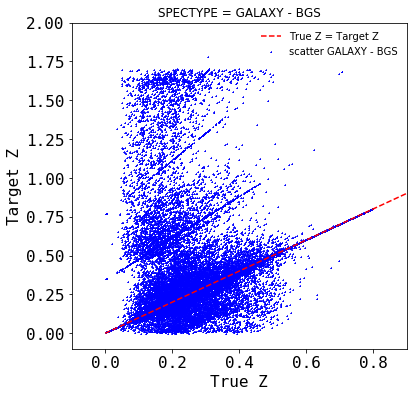
\includegraphics[width=1\linewidth]{TeX_files/Imagenes/BGS-z-truez}
		\caption{}
		\label{fig:BGS-z-truez} 
	\end{subfigure}    
	\begin{subfigure}[b]{0.5\textwidth}
		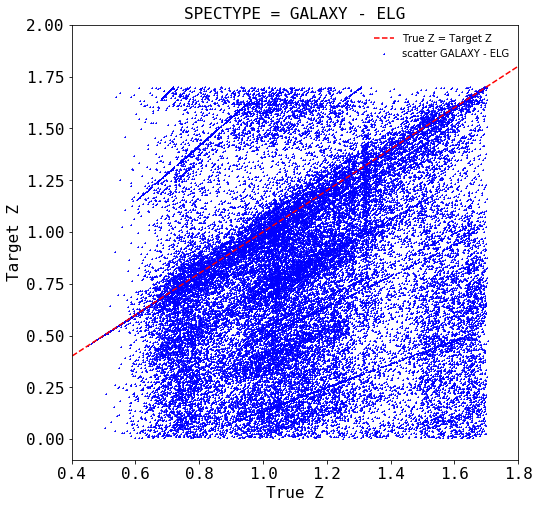
\includegraphics[width=1\linewidth]{TeX_files/Imagenes/ELG-z-truez}
		\caption{}
		\label{fig:ELG-z-truez}
	\end{subfigure}
	\begin{subfigure}[b]{0.5\textwidth}
		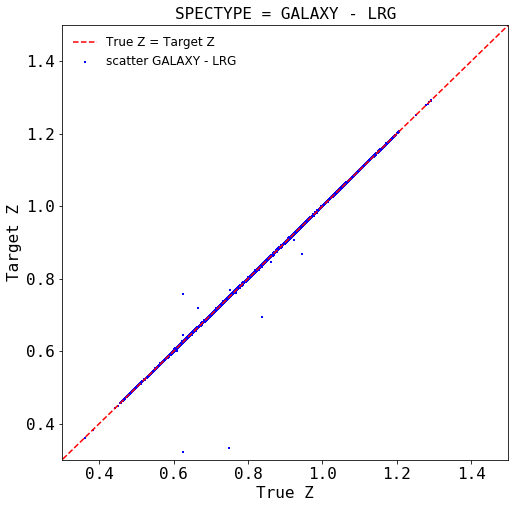
\includegraphics[width=1\linewidth]{TeX_files/Imagenes/LRG-z-truez}
		\caption{}
		\label{fig:LRG-z-truez}
	\end{subfigure}
	\caption{ Redshift relation for Galaxy (a) BGS-type objects, (b) ELG-type objects, and (c) LRG-type objects }
	\label{fig:GALAXY-SUB-z-truez}
\end{figure}

\section{Relevant Features}
The ability of the instrument for measuring the correct redshift will probably depend on the quality of the fluxes that the fiber optics receive. The fluxes of the objects are related to its magnitude, as we saw in Figure \ref{fig:mag-dist-both}, the magnitude is related to the correct prediction of the instrument's Z, but since the information of magnitude is known to the instrument in form of fluxes, this variables will be explored next. The six fluxes variables are named in Table \ref{tab:tar_car}.  The distributions of the fluxes in the BGS dataset are shown in Figure \ref{fig:bgs-flux-dist}.

\begin{figure}[h!]
	\centering
	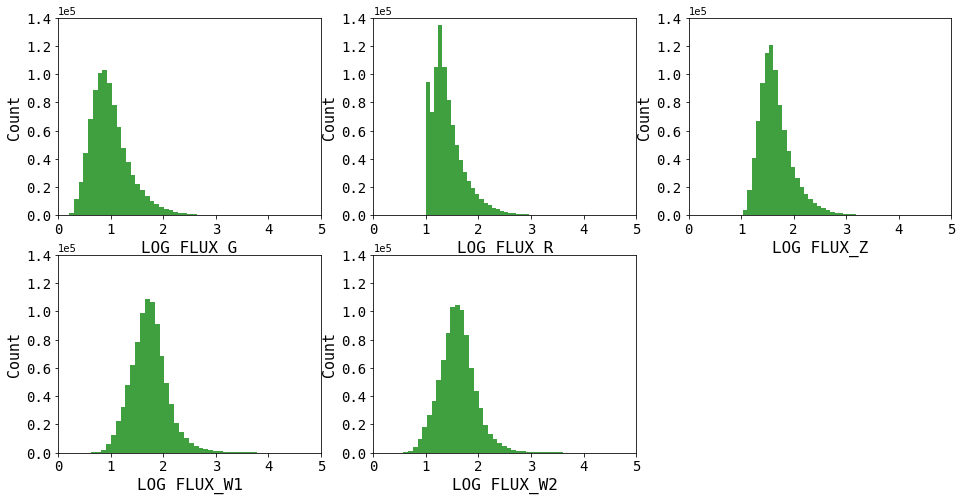
\includegraphics[width=1\linewidth]{TeX_files/Imagenes/BGS-flux-dist}
	\caption{Distribution of the flux variable in the BGS subset.}
	\label{fig:bgs-flux-dist}
\end{figure}

In order to keep track of the relation between TARZ y TRUEZ and see the behavior of the flux variable with respect to the two, we define the following variable
\begin{equation}
\alpha = \frac{TRUEZ}{TARZ},
\end{equation}
therefore, alpha have a value near 1 when the redshifts are along de 45-degree line. 
\begin{figure}[!htp]
	\centering
	\begin{subfigure}[t]{0.5\textwidth}
		\centering
		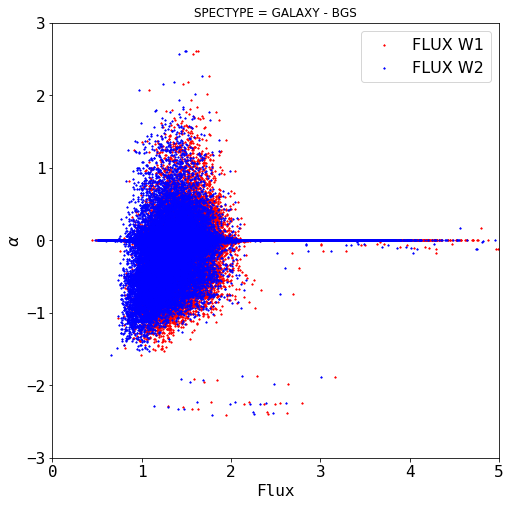
\includegraphics[height=3in]{TeX_files/Imagenes/BGS-FLUXW-ALPHA}
		\caption{}
	\end{subfigure}%
	\begin{subfigure}[t]{0.5\textwidth}
		\centering
		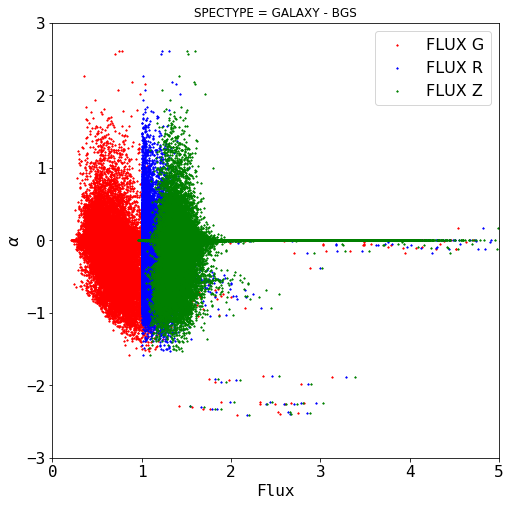
\includegraphics[height=3in]{TeX_files/Imagenes/BGS-FLUXRGZ-ALPHA}
		\caption{}
	\end{subfigure}
	\caption{Relation between fluxes, TRUEZ and TARZ. (a) $\alpha$ as a function of W1 and W2 fluxes. (b)$\alpha$ as a function of G, R and Z fluxes. $\log_{10}$ values presented.}
	\label{fig:BGS-FLUX-ALPHA}
\end{figure} 

We see in Figure \ref{fig:BGS-FLUX-ALPHA} that each flux has a similar behavior, however, they are dispersed in different values and present different minimum values. As the flux magnitude increases, $\alpha$ tends to equal 1, meaning that as the fluxes received by the instrument increases, the redshift measurements are closer to the expected real values. Therefore, the dispersion regions may contain the information necessary for the ML models to learn no predict better redshifts. To see the influence of the dispersion at low fluxes over $\alpha$, the cuts at different fluxes values in Figure \ref{fig:flux_cut_alpha} show the distribution of $\alpha$ at particular values of the fluxes. 
\begin{figure}[h!]
	\centering
	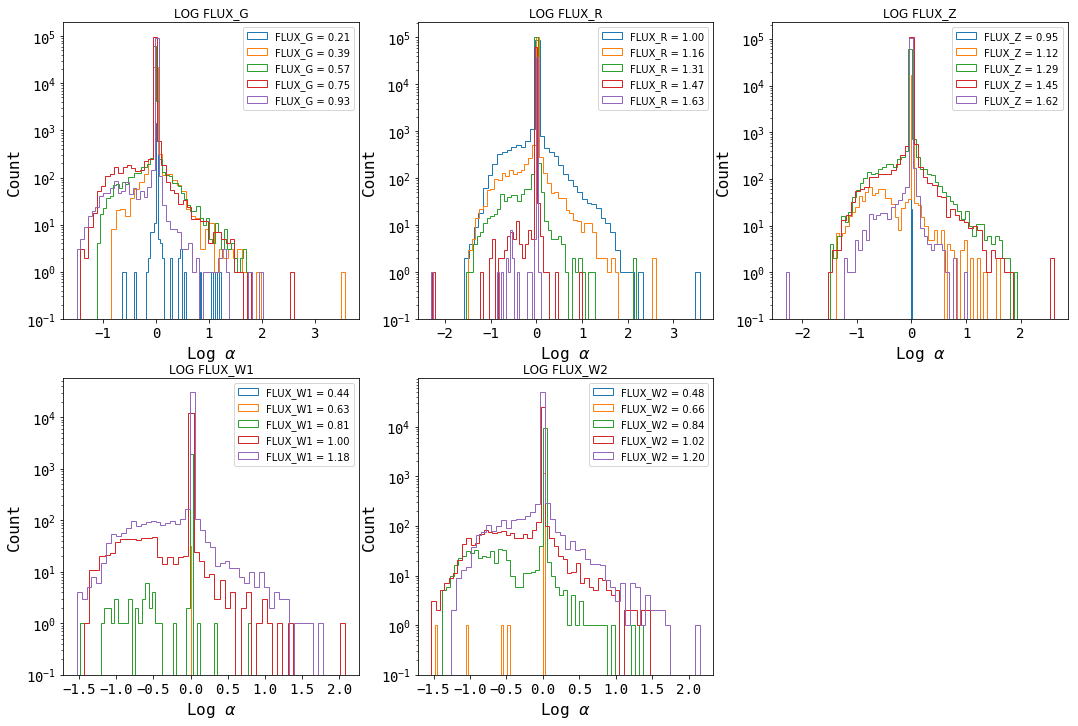
\includegraphics[width=1.0\linewidth]{TeX_files/Imagenes/flux_cut_alpha}
	\caption{Distribution of $\alpha$ at different cuts in the flux variable from figure \ref{fig:BGS-FLUX-ALPHA}}
	\label{fig:flux_cut_alpha}
\end{figure}

The plots in Figure \ref{fig:flux_cut_alpha} are constructed by taking thin slices at fixed values of the fluxes in Figure \ref{fig:BGS-FLUX-ALPHA} and constructing the histogram of the points that lie within the slice. The first approximation is to fit the distribution to a Gaussian distribution and estimate its mean and variance. The relation between mean and fluxes is shown in Figure \ref{fig:media_alpha_flux}, were the green points indicate the mean of $\alpha$ for the slice taken at the given flux. The blue line in Figure \ref{fig:media_alpha_flux} indicates when $TRUEZ = TARZ$, therefore, we see in that for each flux, there are ranges within $\mu(\alpha)$ is not 1, even when the typical error is small. These ranges are around 1 (in log scale) for all the fluxes. Also, note that at very high fluxes, the error in the mean increases, related to the fewer data available at those values and its high dispersity. 
\begin{figure}[!htbp]
	\centering
	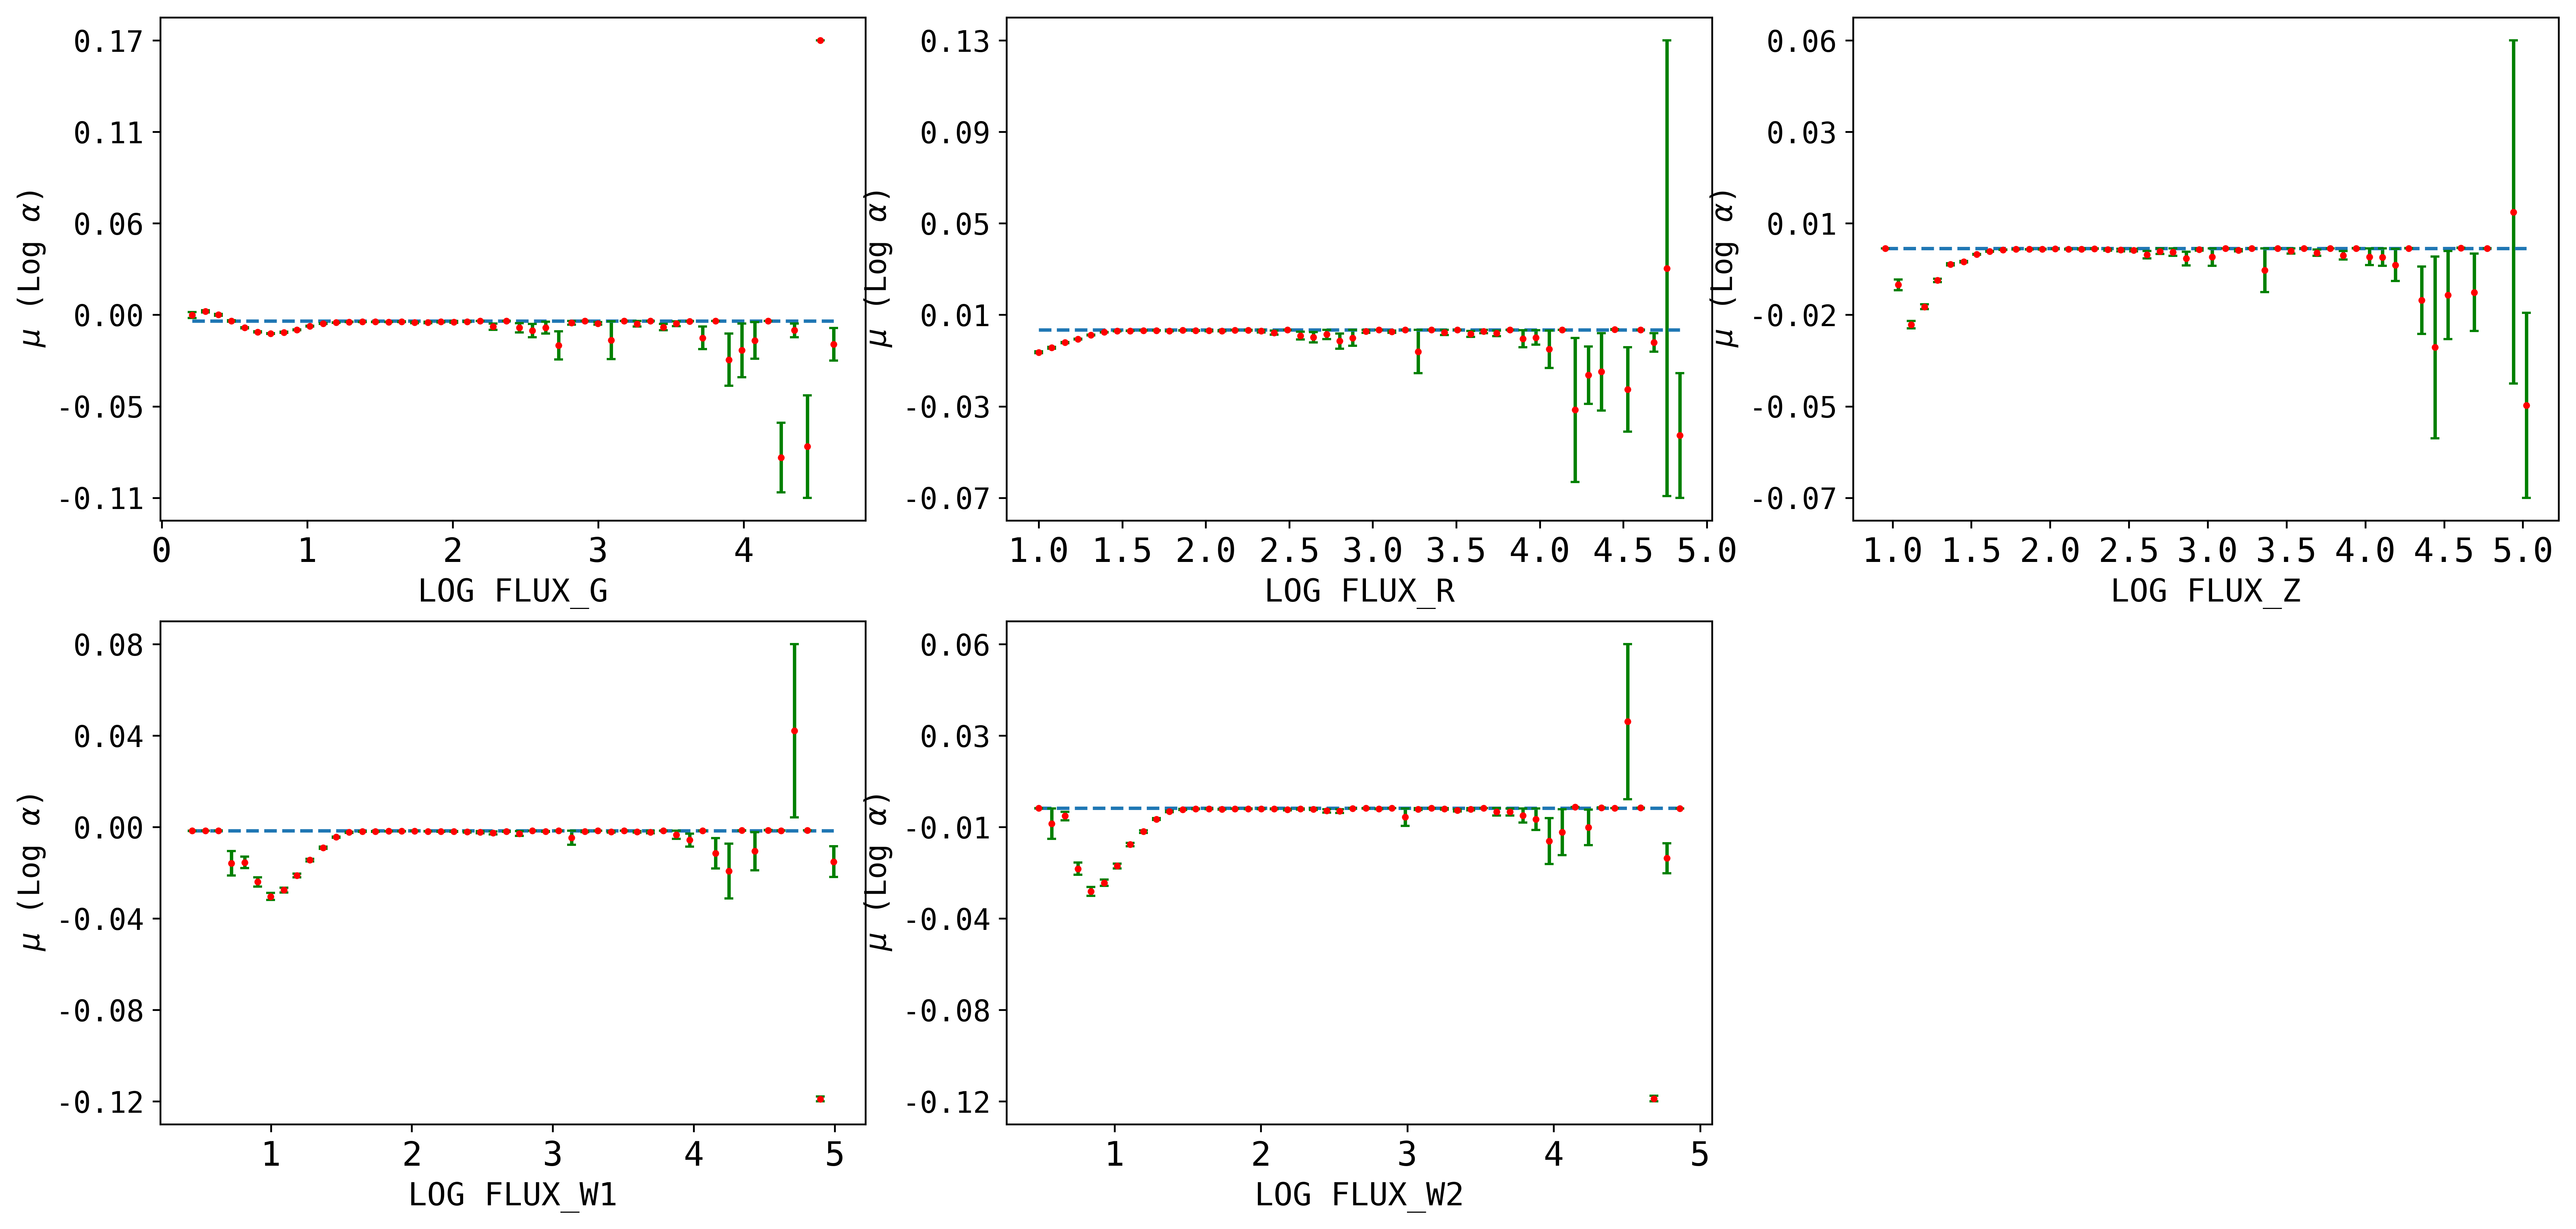
\includegraphics[width=1.0\linewidth]{TeX_files/Imagenes/media_alpha_flux}
	\caption{Mean (red) and standard error (green) of $\log_{10}(\alpha)$ for every Flux interval (slice).}
	\label{fig:media_alpha_flux}
\end{figure}

\section{Conclusions}
The dataset consists of two sets of simulated observation, the truth-file, with the simulated expected results of redshifts (TRUEZ) from the survey targets, and the target-file with the simulated observations by the instrument of the targets redshifts (TARZ). The targets are classified as Galaxies, QSOs and Stars, being Galaxies the most representative type with 84.25\% of the dataset. From this, the most interesting subtype of galaxies is the Bright Galaxy Survey (BGS) because of its patterns in redshift and the amount of data (49.51\% of the Galaxy type). The results in the following chapter are focused only in the BGS subtype, using as input features for the machine learning algorithms the fluxes and the target redshift, and as output the true redshift. 